\documentclass{standalone}
\begin{document}
	\subsection{Lung Extraction}
	
	This script aims to achieve the HU registration, the lung segmentation and the bronchial removal. 
	
	The lung mask was created by applying the suitable method from~\cite{REP:lungmask}. 

	In order to achieve the first step, first of all all the values less than the air value are setted to this value, after that the air value is subtracted from all the voxels. These operation are performed on the image tensor by using \textsc{Numpy} ndarray method.  
	
	\lstset{style=python}
	\begin{lstlisting}[language=python, caption=HU registering function, label=code:saf]
		
	import numpy as np
		
	def shif_and_crop(tensor) :
		
		tensor[tensor <  -1024] = tenor[tensor > -1024].min()
		tensor = tensor - tensor.min()
	
		return tensor
	\end{lstlisting}

	More inreresting is the estimation of the eignevalues map. To achieve this purpose I've implemented a function based on \textsc{cv2.cornerEigenValsAndVec} in \textsc{OpenCV}. This function takes as input an $8-$bit gray scale image, so we have to rescale the GL value of the obtained image tensor. Since I don't want to lose information about the rescaled values, I've simply made a copy of this object. 
	
	In the end the computing of the eigenvalues map is made by the following function: 
		\lstset{style=python}
	\begin{lstlisting}[language=python, caption=HU registering function, label=code:saf]
		
	import cv2
	import numpy as np
	from functools import patial
		
	def max_eigenvalues_map(tensor, block_size, kernel_size) :
		
		func = partial(cv2.cornerEigenValsAndVecs, 
						blockSize = block_size, 
							ksize = kernel_size)
		res = np.array(list(zip(*list(map(func, tensor)))))
		res = res.transpose(1, 0, 2, 3)
		res = res[:, :, :, :2]
		max_eigenvals = np.max(res, axis = 3)
	
		return max_eigenvals

	\end{lstlisting}

	Once the required parameter were setted, the \textsc{OpenCV} function is iterate over the axial slices. The following transposition and selection of tensor elements, are needed since the function returns also the eigenvectors, in which we are not interested in. 
	
	At the end of the whole procedure, the resulting tensor is saved into a medical image formats. In this step I have paid attention to preserve also spatial informations.
	
	

	%This is a pre-processing step, which involves the creation of a lung mask and the managing of the Hounsfield Unit. The creation of a mask for the lung regions aims to reduce the number of clusters and avoid the formation of false positives by removing external structures, which can be source of errors. In order to achieve this purpose, I have decided to use a pre-trained neural networks~\cite{REP:lungmask} which code is open source. 
	
	%\textbf{red}{Once we have found a suitable mask for the lung, a managing of HU must be performed. The $k$ constant in the HU definition (equation\,\ref{eq:HU}) may change according to the scan manufacturer or scan model; moreover, during the scan acquisition, all the regions outside the CT tube aren't sampled, so to obtain a square $N\times N$ image for each slice some padding values are added, which different values according to the scan manufacturer: for instance in the CT scan in \figurename\,\ref{fig:Pre-Processing}(a) the padding value is $-3000 HU$ and the air value is $-1024$. }
	
	%The first thing to do is to make the padding value and the air value equal for each scan considered and shift them to $1$: in this way we have registered the HU for scan from different manufactures in a common space, as we can see in \figurename\,\ref{fig:Pre-Processing}(b).
	
	 %May happen that some patients have metallic prothesis, so metallic artifact may be present. Since usually this implant are outside the lung, are removed after the mask application, so no other step are needed.
	 
		%\begin{figure}[h!]
		%\centering
		%%\subfigure[Histogram of a CT scan before registration]
	%	{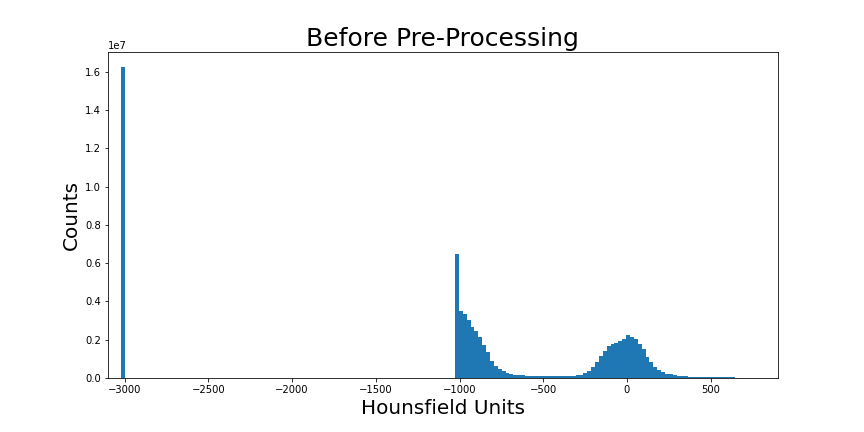
\includegraphics[scale=.3]{HU_before_rescaling.png}}
	%	%\hspace{1mm}
	%	\subfigure[Histogram of a CT scan after the registration]
	%	{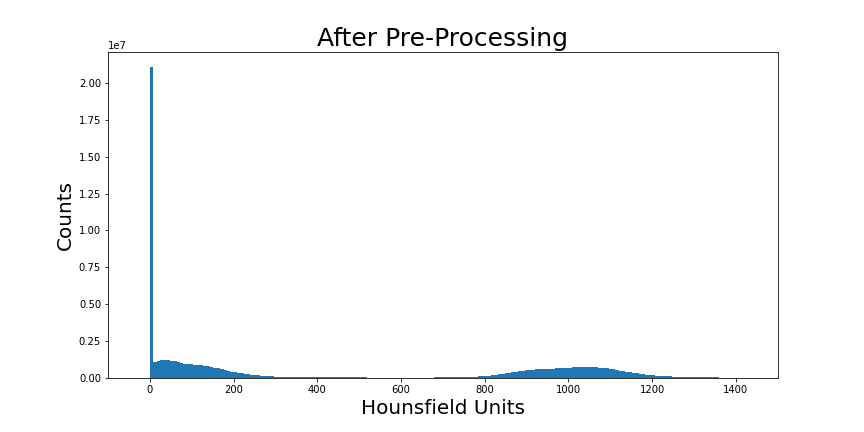
\includegraphics[scale=.3]{HU_after_rescaling.png}}
	%	\caption{Histogram of voxel values before and after the pre-processing. We can observe that before the pre processing there are some HU out of range, which are the values used to fill the regions outside the tube, and the air value is around $-1000\,HU$ according to HU definition. After the rescaling we can observe that all the values are non-negatives.}\label{fig:Pre-Processing}
	%\end{figure}
	%Now, we have found the mask for the lung regions, and we have managed the HU, so by a simple element wise AND we are able to isolate the lung from the rest of the body, removing also the organs, like heart and intestine, presents in the CT scans.
	
	%We have observed that the presence of the bronchial structure in the lung regions is one of the main source of false positives, so an extra step was added in order to remove as much as possible this kind of structures.
	
	 %Bronchi have an elongated shape respect to the other structure which usually are rounded: the basic Idea was to use this kind of information, by using the \href{https://www.docs.opencv.org/master/dd/d1a/group__imgproc__feature.html#ga04723e007ed888ddf11d9ba04e2232de}{cornerEigenValsAndVecs} function implemented in \textsc{OpenCV}. This particular filter compute the covariant matrix of the derivative in a neighborhood and the corresponding eigenvalues. If a particular regions has an elongated shape, one of the eigenvalues (corresponding to the eigenvector in the direction of the structure) will have an higher value, otherwise both eigenvalues have a lower value. So we have applied this filter on each slice of the scans and took the maximum eigenvalues. 
	%\begin{figure}[h!]
	%	\centering
	%		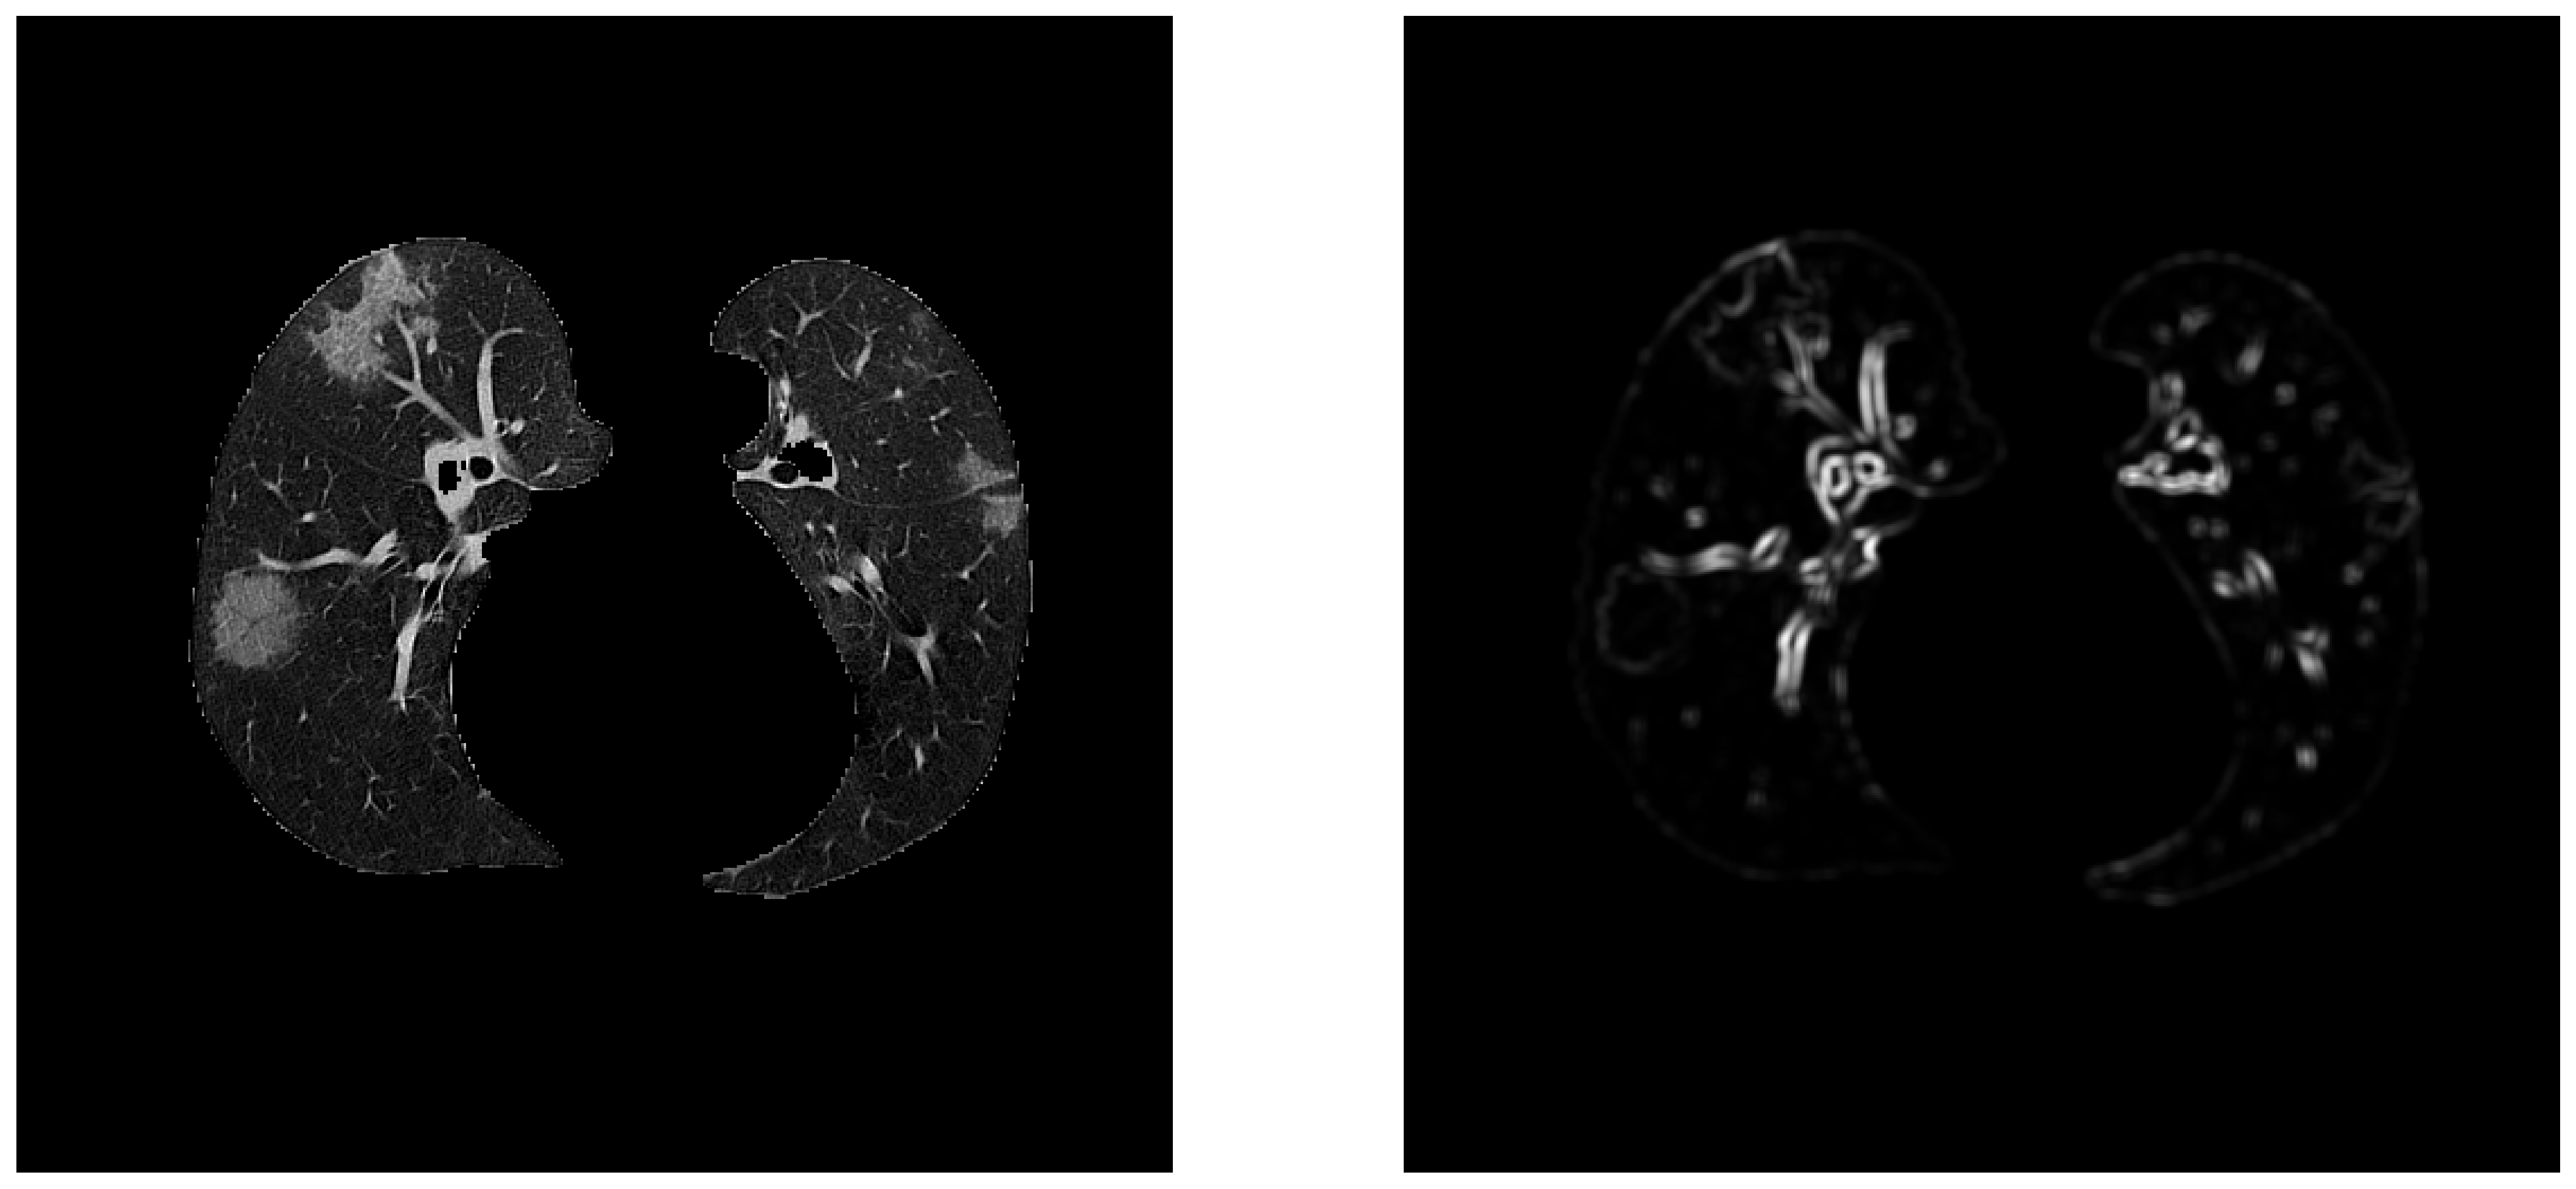
\includegraphics[scale=.3]{MaxEigenVal.png}
	%		\caption{From left to right: lung regions selected by the U-Net; ,maximum eigenvalues map of the lung. As we can see the U-Net does not exclude the bronchial structure from the lung, on the other hand, the maximum eigenvalues map delineates very well these regions.We have used this map to remove the unwanted bronchial regions.}\label{fig:MaxEigenval}
	%\end{figure}

	%In \figurename\,\ref{fig:MaxEigenval}, I've displayed the image after the lung segmentation by the neural network, and the corresponding eigenvalues map. As we can see the higher values of the map corresponds to the edges of the main bronchial structures. To create the mask for these structures a simple threshold on the map was taken. Since the main bronchial structures are large, this process is able to remove only part of the edges, but the inner structure is preserved. In order to refine the segmentation, this process is repeated a second time, allowing a more accurate exclusion of the structures.
			
\end{document}